
\section{Spatial Closure Based on the HO Solution}
\label{sec:spat_clos}

This sections describes an alternative spatial closure to the LO equations with
a parametric relation determined with the HO solution. In addition to estimating the angular
consistency terms, the HO intensity is used to estimate a relation between volume and face-averaged
intensities to eliminate the face unknowns from the LO equations. 
 The goal is to improve consistency compared to the LDFE discretization, although
additional statistical noise is introduced through face-based tallies.
In the remainder of
this section, we motivate the HO spatial closure by manipulating a half-range balance
equations to form a single unknown for each cell and half range.  We will then discuss
the forms of HO spatial closures investigated, based on modifications to standard spatial closures.

\subsection{Motivation}

Independent of angular accuracy and convergence of outer iterations, the LDFE closure of the LO equations will generally
not produce the same moments as the LDFE projection of the HO solution.  As an example of
this difference, in the LO equations the linearly extrapolated outflow from one cell is defined as the
inflow into the next cell through upwinding.  For the HO solver, the linear,
projected MC outflow from a spatial cell does not not match the actual energy
that flowed into a downstream cell via MC particles.  Thus, we introduce additional
unknowns at the face of cells to exactly capture the relation between moments and face
values.

A half-range balance equation for $\mu>0$ is formed by adding the
exact $L$ and
$R$ radiation moment equations given by
Eq.~\eqref{eq:exact_lmomp}~and~\eqref{eq:exact_rmomp}, i.e.,
\begin{equation}\label{eq:hr_bal}
    \mu^+_{i+1/2}\phi_{i+1/2}^+ - \mu^+_{i-1/2}\phi_{i-1/2}^+ +
    {\sigma_{a,i}h_i} \phi_i^+ = \frac{h_i}{2} q_i,
\end{equation}
where $q_i$ represents the cell-averaged emission source.  In the HOLO algorithm, after
estimating the consistency terms $\mu_{i\pm1/2}^+$ upwinding the inflow term
$\phi_{i-1/2}^+$, an additional equation is needed to eliminate the outflow $\phi_{i+1/2}^+$ to produce an
equation for a single unknown $\phi_{i}^+$.  Standard spatial discretizations techniques
use a fixed approximation for all cells to eliminate the outflow in terms of other
unknowns.  Alternatively, the HO solution can be used to estimate a parametric relation
between the other unknowns and the outflow, i.e.,
\begin{equation}\label{eq:ho_clos}
    \phi_{i+1/2}^+ = f(\gamma^{+,HO}_i, \phi_i^+, \phi_{x,i}^+, \phi_{i-1/2}^+),
\end{equation}
where $\gamma^{HO,+}_i$ is a local constant to be estimated with the HO solution and $f$ is some
function of some number of the input
variables.  The ECMC solution can provide all of the unknowns in the above equation, so
the value of $\gamma^{HO}_i$ can be determined directly. 

If the problem were linear, or the nonlinear problem was fully converged,
then application of this closure can ensure that the HO and LO equations produce the same
moments, preserving the HO accuracy.  To produce the
same zeroth moment, the HO solution must also satisfy the local balance equation, e.g.,
Eq.~\eqref{eq:hr_bal}.  Then the LO equations and HO equations will have the same moments
to satisfy both Eq.~\eqref{eq:ho_clos} and Eq.~\eqref{eq:hr_bal}, upon nonlinear
convergence of the outer HOLO iterations. To accurately reproduce the $L$ and $R$ basis
moments, then the HO and LO solutions must also satisfy the first moment equation.

As TRT problems are non-linear (i.e., scattering or thermal emission are included in
$q$), the moments will only be preserved upon non-linear convergence of the source.  The
nonlinearity introduces the possibility for stability
issues, particularly with MC noise.  However, we have already consistently formed angular consistency terms, so the
the spatial closure should be more stable than introducing auxiliary terms, such as
in NDA methods~\cite{rmc,willert}, but has a higher memory cost per spatial cell. 

\subsection{Choice of Spatial Closure}
\label{sec:spat_clos_options}

We will
explore two different closure relations based on modifications to the standard LD closure: a scaled slope, i.e.,
\begin{equation}\label{eq:cl_slope1}
    \phi_{i\pm1/2}^\pm = \phi_i^+ \pm \gamma_i^{\pm} \phi_{x,i}^+
\end{equation}
and a scaled average
\begin{equation}\label{eq:cl_avg1}
    \phi_{i\pm1/2}^\pm = \gamma_i^{\pm} \phi_i^+ \pm \phi_{x,i}^+,
\end{equation}
where a value of $\gamma_i = 1$ produces the standard linear discontinuous expressions for
the extrapolated outflows.  Our LO system is formulated in terms of $L$ and $R$ moments, rather than the average and
slope.  Thus, Eq.~\eqref{eq:cl_slope1} and~\eqref{eq:cl_avg1} are expressed in terms of the $L$ and $R$
unknowns, using the relations given in App.~\ref{app:lo_mom_relations}.  In terms of these
moments, the scaled-slope closure is
\begin{align}\label{eq:cl_slope}
    \phi_{i+1/2}^+  &= \left(\frac{\ds 1 - 3 \gamma_i^+}{\ds 2 }  \right)
    \mom{\phi}_{L,i}^+ + \left(\frac{\ds 1 + 3 \gamma_i^+}{\ds 2 }  \right)
    \mom{\phi}_{R,i}^+ \\
    \phi_{i-1/2}^-  &= \left(\frac{\ds 1 + 3 \gamma_i^-}{\ds 2 }  \right)
    \mom{\phi}_{L,i}^- + \left(\frac{\ds 1 - 3 \gamma_i^-}{\ds 2 }  \right)
    \mom{\phi}_{R,i}^- 
\end{align}
and the scaled-average relation is
\begin{align}\label{eq:cl_avg}
    \phi_{i+1/2}^+  &= \left(\frac{\ds  \gamma_i^+ - 3}{\ds 2 }  \right)
    \mom{\phi}_{L,i}^+ + \left(\frac{\ds \gamma_i^+ + 3}{\ds 2 }  \right)
    \mom{\phi}_{R,i}^+ \\
    \phi_{i-1/2}^-  &= \left(\frac{\ds \gamma_i^- + 3}{\ds 2 }  \right)
    \mom{\phi}_{L,i}^- + \left(\frac{\ds \gamma_i^- - 3}{\ds 2 }  \right)
    \mom{\phi}_{R,i}^- .
\end{align}
%REWRITE: May add results for ratio of average
%It is tempting to use a closure that is only a function of the average.  This
%Although this can produce accuracy in smooth problems, it leads to a problem where the
%slope of the source is accounted for almost entirely in the slope of the radiation and the
%outflow is not forced to do anything intelligent. If you had scattering, this would become
%very inaccurate.  This can be seen by looking at marshak wave and the slope equation, as
%you come to equilibrium it causes problems.

The HO solution is used to estimate $\gamma_i$. The MC solution must be modified
to tally the MC estimated intensity on faces. For example, for $\mu>0$, the LO equations for
moments at $k+1$ use closure parameters evaluated at $k+1/2$ as
\begin{equation}
    \gamma_{i}^{+,k+1} = \frac{\phi_{i+1/2}^{+,k+1/2} -
    \phi_{i}^{+,k+1/2}}{\phi_{x,i}^{+,k+1/2}},
\end{equation}
for the scaled-slope closure.  For this closure, as the slope goes to zero this expression
becomes undefined.  In cells where the slope is $O(10^{-13} \psi_i)$, we use $\gamma_i=1$.
The main benefit of the scaled-slope closure is it allows for values of $\gamma$ that are
equivalent to other closures, as discussed in App.~\ref{app:lo_mom_relations}:
$\gamma_i=0$ produces a step closure~\cite{larsen_edl}, which has a zero slope over the cell, and $\gamma_i=1/3$
produces a lumping-equivalent closure. 

\subsection{The Linear Doubly-Discontinuous Trial Space}
\label{sec:ldd}

Because of the temperature unknowns and the HO scattering source representation, a
representation on the interior of the cell for the temperature and intensity is needed for
construction of sources in the HO solver.
Thus, we introduce a linear doubly discontinuous (LDD) trial space
for the half-range intensities, which is depicted in Fig.~\ref{fig:ldd_space}.  The linear
relation on the interior of the cell preserves the $L$ and $R$ moments of the solution,
and the outflow from the cell is some parametric (i.e., non linear) extrapolation of
those moments. 
The temperature is still represented with a linear interpolant of $T^4$ and $T$.  This
trial space has an extra unknown in the radiation equations for each cell and direction, which is eliminated
from the system with the HO spatial closure.  The ECMC algorithm is modified to also
include a LDD trial space which allows for estimate of the solution at faces, as discussed
later in Sec~\ref{sec:ldd_mc}. 

\begin{figure}[H]
    \centering
    {\resizebox{0.5\textwidth}{!}{
        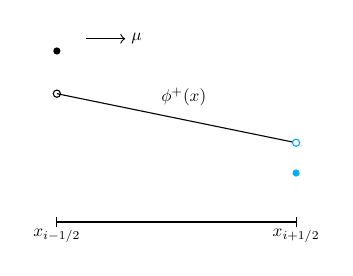
\begin{tikzpicture}[scale=0.62, every node/.style={transform shape}]
            \draw (1.0,4.0) node[fill,circle,inner sep=0pt,minimum
            size=4.2pt] {};
            \draw [->] (1.6,4.25) -- (2.4,4.25) node[anchor=west] {$\mu$};
            \draw (1.0,0.4) -- (1.0,0.6) node[below, pos=0.4] {$x_{i-1/2}$};
            \draw (5.90,0.4) -- (5.90,0.6) node[below, pos=0.4] {$x_{i+1/2}$};
            \node at (3.6,3.06) {$\phi^+(x)$};
            \draw [thick] (1.0,0.5) -- (5.9,0.5) node[anchor=north west] {};
            \filldraw[color=black, fill=white] (1,3.1250) circle (2.1pt);
            \draw (1.0,3.125) -- (5.90,2.120);
            \filldraw[color=cyan, fill=white] (5.9,2.120) circle (2.1pt);
            \draw (5.9,1.5) node[cyan,fill,circle,inner sep=0pt,minimum size=4.2pt] {};
        \end{tikzpicture}
    }}
    \caption{Linear doubly-discontinuous representation for mean intensity in LO equations.     \label{fig:ldd_space}}
\end{figure}

To solve the LO equations, Eq.~\eqref{eq:cl_slope} or~\eqref{eq:cl_avg} is substituted
locally for
the appropriate outflow face term in each LO moment equation. There is a spatial closure parameter for each
half-range, for each cell.
 The $\gamma_i^\pm$ are
estimated from the previous HO solution. For the initial LO solve within each
time step, the outflow is assumed continuous, using the standard upwinding and LD closure.  
As an example, the positive half-range and $L$ moment equation (i.e.,
Eq.~\eqref{eq:exact_lmomp}), for the scaled-slope closure, becomes
\begin{multline}
    -2{\mu}_{i-1/2}^{n+1,+} \left[\left(\frac{\ds 1 - 3 \gamma_{i-1}^{HO,+}}{\ds 2 }  \right)
        \mom{\phi}_{L,i-1}^+ + \left(\frac{\ds 1 + 3 \gamma_{i-1}^{HO,+}}{\ds 2 }  \right)
    \mom{\phi}_{R,i-1}^+
    \right] \\ + \cur {\mu}_{L,i}^{n+1,+}
  \mom{\phi}_{L,i}^{n+1,+}
  +  \cur\mu_{R,i}^{n+1,+}
  \mom{\phi}_{R,i}^{n+1,+}\\ +  \left(\sigma_{t,i}^{n+1}+\frac{1}{c \Delta t} \right) h_i 
  \mom{\phi}_{L,i}^{n+1,+} -  \frac{\sigma_{s,i} h_i}{2} \left( \mom{\phi}_{L,i}^{n+1,+} +
  \mom\phi_{L,i}^{n+1,-}\right)\\  = \frac{h_i}{2} \mom{\sigma_a^{n+1} a c T^{n+1,4}}_{L,i} +
  \frac{h_i}{c\Delta t}\mom{\phi}_{L,i}^{n,+},
    \label{eqn:clsd_posl}
\end{multline}
and the $R$ moment equation becomes
\begin{multline}
    2{\mu}_{i+1/2}^{n+1,+} \left[
    \left(\frac{\ds 1 - 3 \gamma_{i}^{HO,+}}{\ds 2 }  \right)
        \mom{\phi}_{L,i}^+ + \left(\frac{\ds 1 + 3 \gamma_{i}^{HO,+}}{\ds 2 }  \right)
    \mom{\phi}_{R,i}^+
    \right]  \\ 
    - \cur {\mu}_{L,i}^{n+1,+}
  \mom{\phi}_{L,i}^{n+1,+}
  -  \cur\mu_{R,i}^{n+1,+}
  \mom{\phi}_{R,i}^{n+1,+} +  \left(\sigma_{t,i}^{n+1}+\frac{1}{c \Delta t} \right) h_i 
  \mom{\phi}_{R,i}^{n+1,+} \\-  \frac{\sigma_{s,i} h_i}{2} \left( \mom{\phi}_{R,i}^{n+1,+} +
  \mom\phi_{R,i}^{n+1,-}\right) = \frac{h_i}{2} \mom{\sigma_a^{n+1} a c T^{n+1,4}}_{R,i} +
  \frac{h_i}{c\Delta t}\mom{\phi}_{R,i}^{n,+}.
    \label{eqn:clsd_posr}
\end{multline}
These equations contain only the original desired radiation moment and LD temperature unknowns.
During the Newton solve, once new half-range
intensities are determined, the temperatures are updated using the same material
energy equations as for the LD closure, i.e., Eq.~\eqref{eq:lo_mat_dis1} and Eq.~\eqref{eq:lo_mat_dis2}.

Because the
outflow from one cell is upwinded into the next cell, energy conservation by the LO
equations is preserved.
The closed equations have the
same numerical complexity as the LDFE LO equations, but with an increased storage on the
coarse mesh for the
$\gamma_i^{\pm}$ values.  The linear representation for the interior
solutions and emission source approaches the LD closure in the equilibrium diffusion limit, as long
as the HO spatial closure is estimated with sufficient statistical accuracy.  


\subsection{Fixup for the Linear Doubly-Discontinuous Trial Space}
\label{sec:ldd_fix}

% For this case, we use the lumped
%representation on the interior of the solution for all cells. The outflow can still be driven negative
%due to non-linearities, which leads to negative values in down-stream cells. 
%This is a result of the HO estimation of the spatial closure using
%moments based on lagged source terms.  
The doubly discontinuous trial space presents an additional difficulty for resolving
negative intensities because the outflow
is now unhinged from the linear relationship. 
In the case of strong gradients, the interior representation and outflow can be driven
negative.  In such cases, we apply the lumping-equivalent relation from
App.~\ref{app:lo_mom_relations} to define the linear representation.  For
example, the lumped emission source is
\begin{equation}
    T = \mom{T}_{L,i}^4 b_{L,i}(x) + \mom{T}_{R,i}^4 b_{R,i}(x) , \quad x\in(\xl,\xr)
\end{equation}
where $T_{L,i}\equiv \mom{T}_{L,i}$ and $T_{L,i}\equiv \mom{T}_{L,i}$ for the lumping closure.
There are analogous relations for $T(x)$ and $\phi^\pm(x)$ over the interior of each cell.
These expressions are positive as long as the moments are positive.  If the lagged, MC spatial closure produces an outflow from a cell that is
negative, then these moments could become negative. 
It is important to note that the spatial closure will still have the same
relation between the moments and the outflow; the lumping relation only affects the
linear representation that the moments correspond to.  For example in the $L$ moment of
the material energy (Eq.~\eqref{eq:lo_mat_dis1}), the lumped representation changes $2/3
T_{L,i} + 1/3 T_{R,i}$ to $T_{L,i}$, but no modifications are made to the
absorption term $\sigma_{a,i}\mom{\phi}_{L,i}$; no modifications are made to
the radiation terms in the radiation moment equations.
%In such cases, we force that cell to
%use a standard lumped relation for the moment equations, with no discontinuity at the
%outflow, and restart that Newton solve.  %During the Newton solve, once new half-range
%intensities are determined, the temperatures are updated using the material energy
%moment equations, i.e., Eq.~\eqref{eq:lo_mat_dis1} and Eq.~\eqref{eq:lo_mat_dis2}. For the
%uulumped case, the radiation moments are the same.  he slope moment,
%e.g., $\psi_{x,i}^\pm$, does not strictly correspond to the slope in the typical since.
%We have modified it in the lumped relation.  This is the same as the lumped closure relation using
%$\gamma_i=1/3$, where we are preserving the average moment exactly, but only second order
%accurate in the slope.




